\section{Simulation Analysis}

\label{sec:simulation}
We ran a simulation of the circuit using {\it Ngspice} thus obtaining the following results, for the currents and voltages in the circuit

\begin{table}[h]
  \centering
  \begin{tabular}{|l|r|}
    \hline    
    {\bf Name} & {\bf Value [A or V]} \\ \hline
    f & 1.004690e+03\\ \hline
gain & 3.652900e+01\\ \hline
z & 1.519501e+03\\ \hline

  \end{tabular}
  \caption{Operating point. A variable preceded by @ is of type {\em current}
    and expressed in Ampere; other variables are of type {\it voltage} and expressed in
    Volt.}
\end{table}
From the operating we can see that both transistors are operating in the forward active region. For the npn BJT, $V_{CE} > V_{BE} $, while for the pnp BJT $V_{EC} > V_{EB}$.

\begin{figure}[!htb]
     \begin{subfigure}[b]{0.48\textwidth}
         \centering
         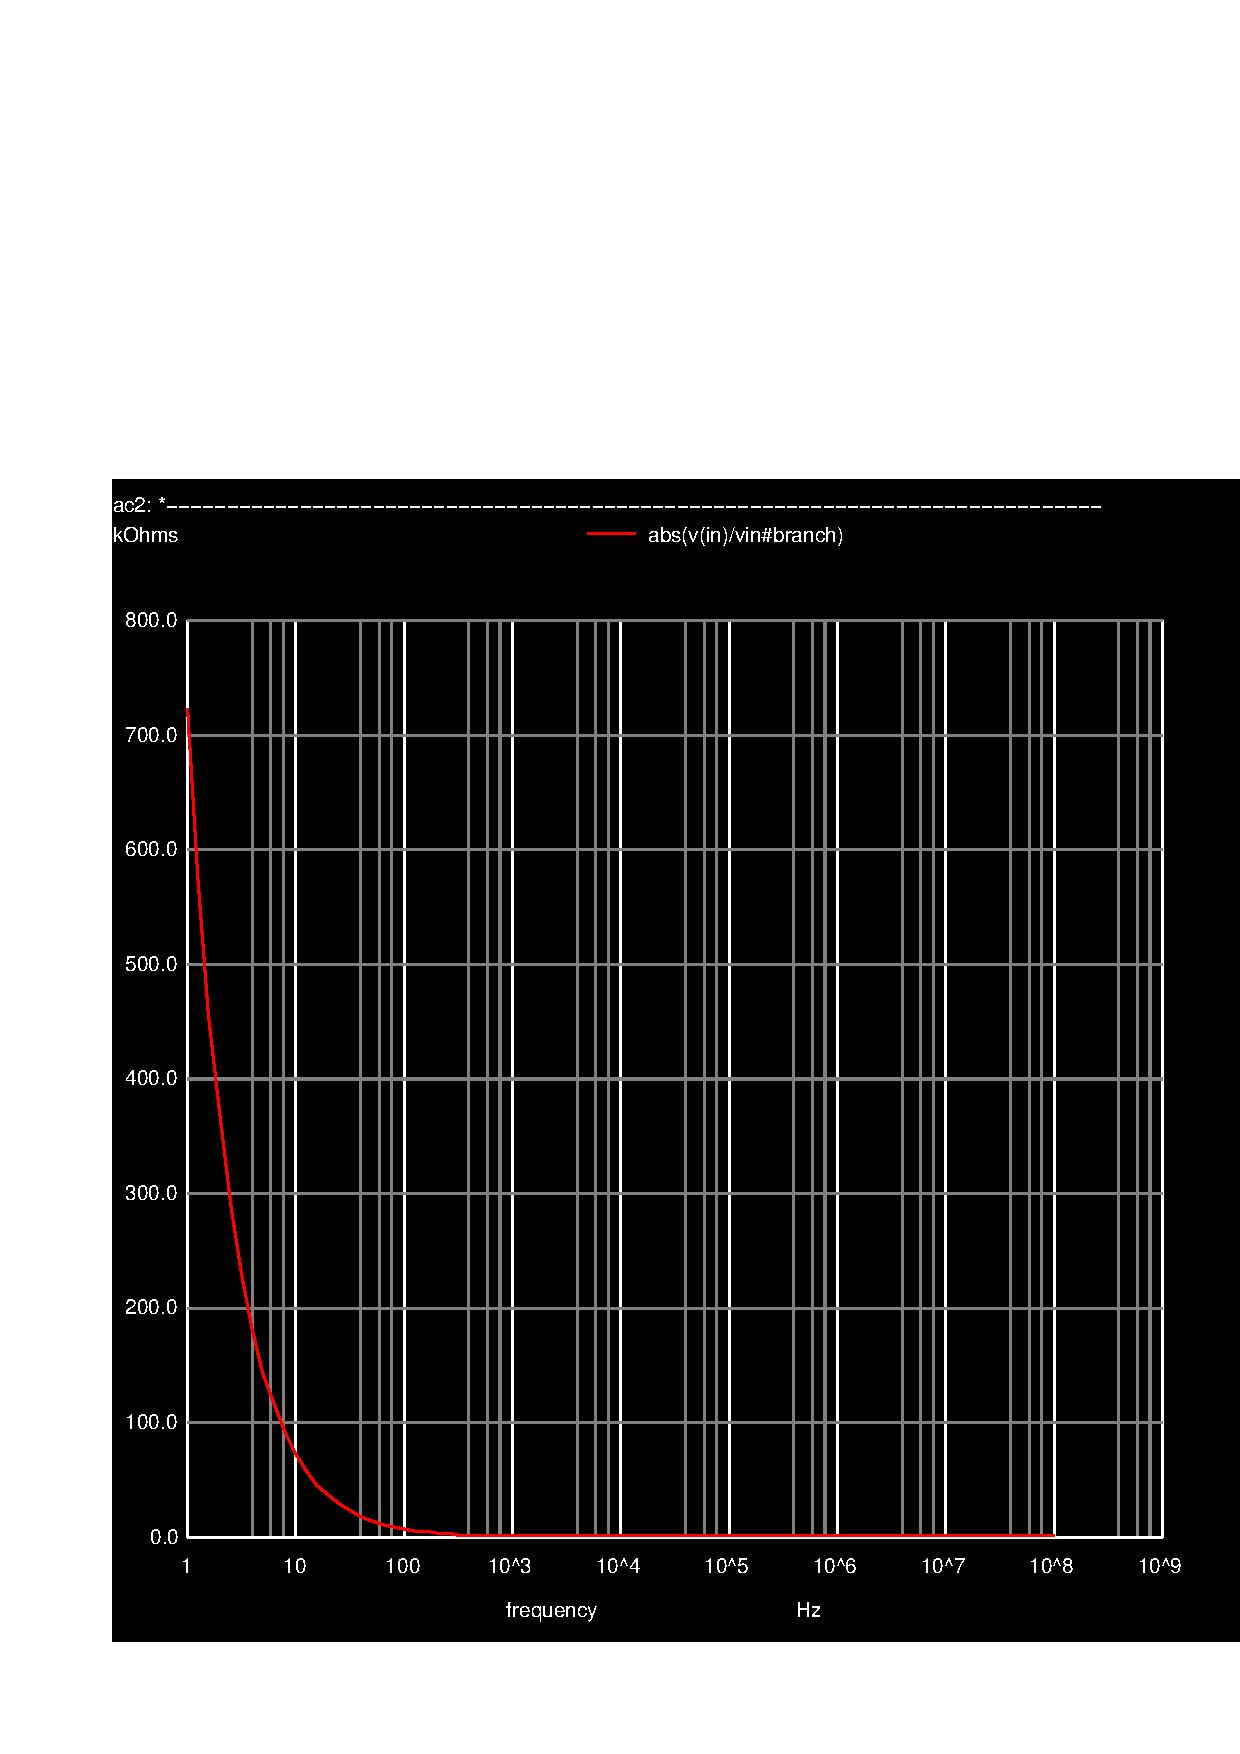
\includegraphics[width=\textwidth]{../sim/1/inputimpedance.pdf}
         \caption{Input impedance of the circuit}
     \end{subfigure}
     \hfill
     \begin{subfigure}[b]{0.48\textwidth}
         \centering
         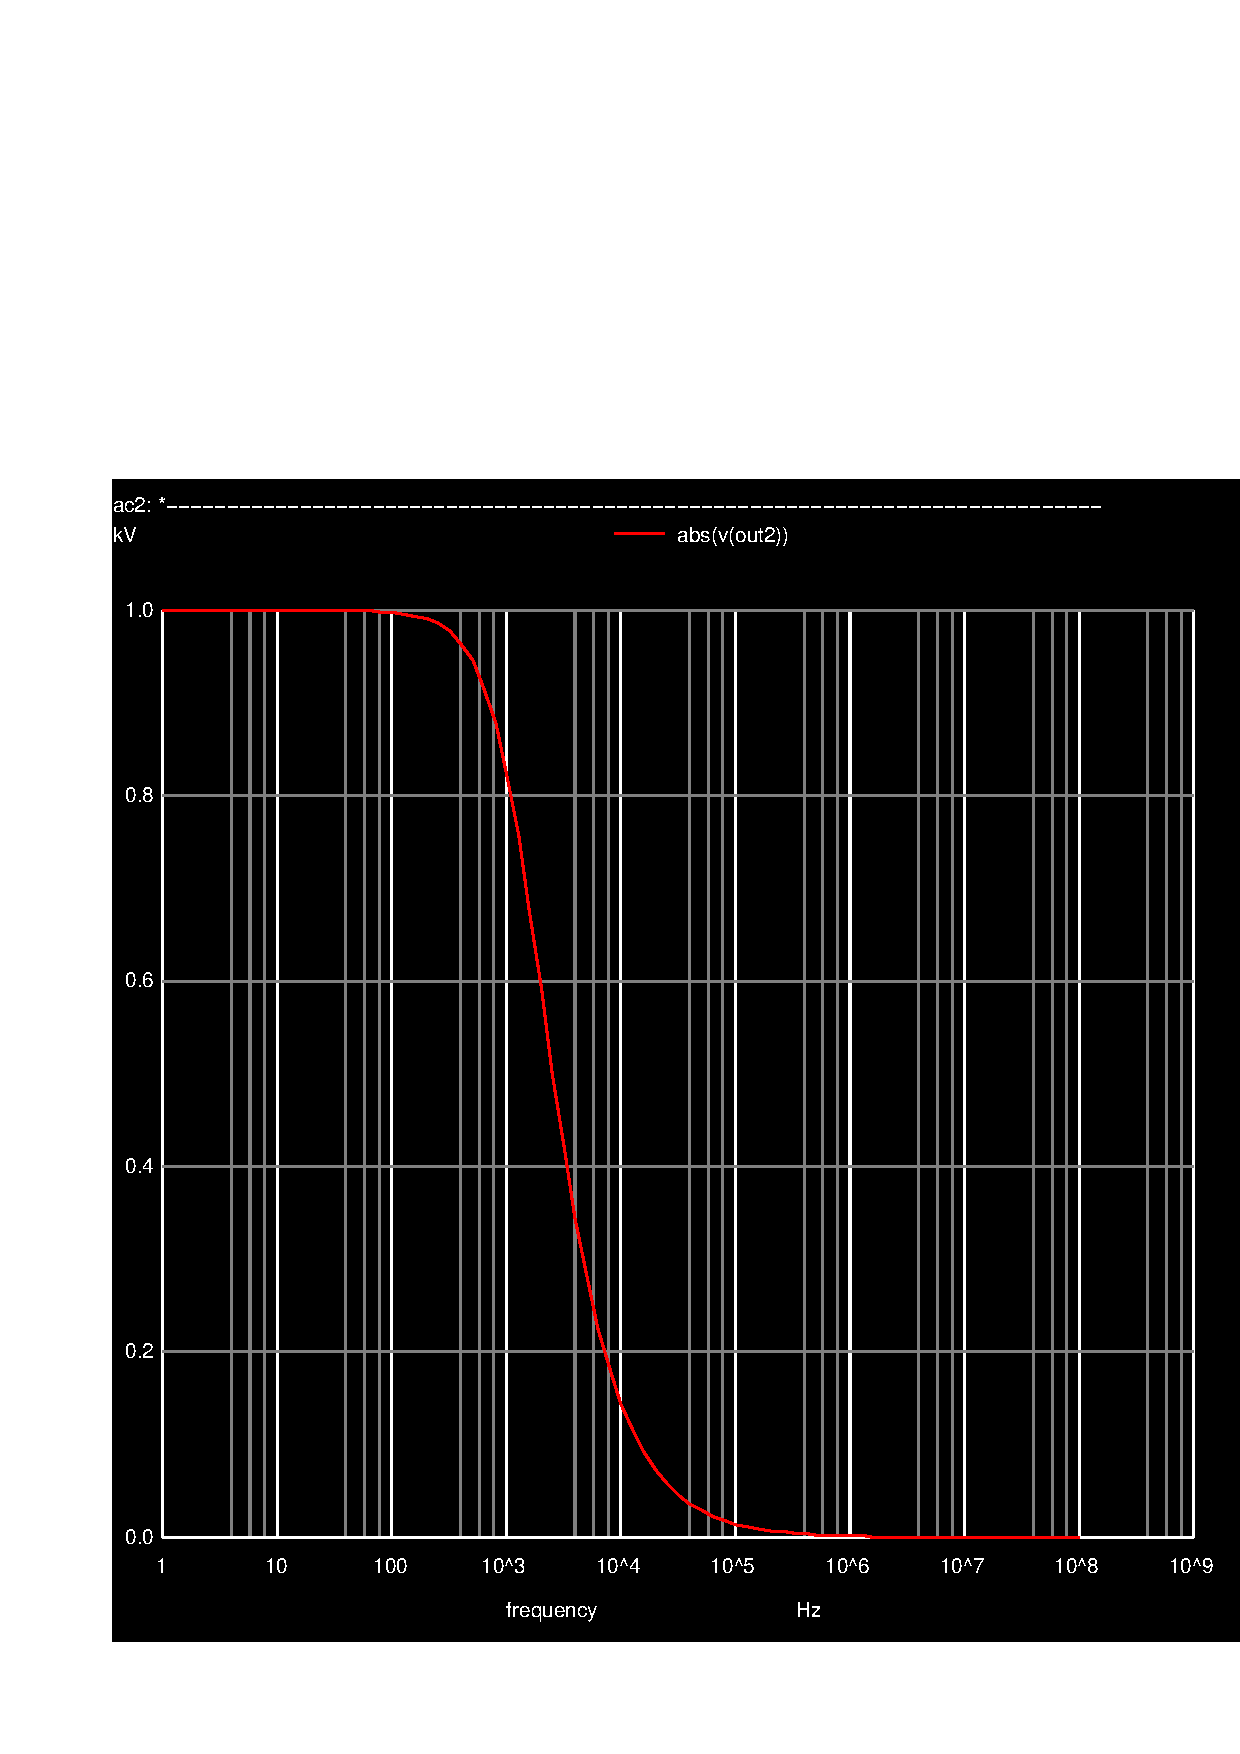
\includegraphics[width=\textwidth]{../sim/2/outputimpedance.pdf}
         \caption{Input impedance of the circuit}
         \label{fig:five over x}
     \end{subfigure}
        \caption{Graphs obtained with \textit{NgSpice}}
        \label{fig:three graphs}
\end{figure}

The output impedance was obtained by conecting an independent current source in series with the capacitor and the other node connecting to ground. The amplitude of the current provided was 1A such that the output impedance was numerically equal to the voltage at the terminals of the current source. Do keep in mind that in order to proprealy mesaure the impedance we fisrt had to short-circuit the input voltage, i.e seting it's amplitude to 0V, besides having removed the load resistor. In a similar way, the input impedance was measured by dividing the input voltage by the current in the branch.In both of the aformentioned procedures \textit{Vcc} was kept on, to mantain the bias of the transistors. 

\begin{figure}[!htb]
     \begin{subfigure}[b]{0.48\textwidth}
         \centering
         \includegraphics[width=\textwidth]{../sim/1/gain.pdf}
         \caption{Gain}
     \end{subfigure}
     \hfill
     \begin{subfigure}[b]{0.48\textwidth}
         \centering
         \includegraphics[width=\textwidth]{../sim/1/vout.pdf}
         \caption{Output signals}
     \end{subfigure}
     \hfill
\end{figure}


The circuit amplifies the signal well for frequencies above 100Hz with a gain of about 35-40 dB, leaving out smaller frequencies of the audible spectrum. Moreover, the gain also diminuishes for higher frequencies (f $>$ 10MHz), which for the audio amplifier should not be a problem, as it is well outside the audible range. The input impedance of the circuit is extremely high for low frequencies and diminuishes progressivly for higher frequencies, as would be expected with the coupling capactior. This feature is very helpful if we want to connect the circuit to a voltage source (whith approximatly infinit impedance). As for the ouput impedance, we have a smillar pattern, but overall low impedance, making the circuit adequate to connect to the $8 \Omega$ load. 
What is more, the output signal shows minimal distortion, as desired to keep the sound intanct.
Finally from the spice simulation we obtained 

  	 
\begin{table}[h]
  \centering
  \begin{tabular}{|l|r|}
    \hline    
    {\bf Name} & {\bf Value [A or V]} \\ \hline
    f & 1.004690e+03\\ \hline
gain & 3.652900e+01\\ \hline
z & 1.519501e+03\\ \hline

  \end{tabular}
  \caption{Cutoff frequencies and Bandwith.}
\end{table}

Hence we obtainned, a merit figure of $2,1 \times 10^7$.
Eventually, the bandwith could be improved by increascing the coupling capacitor, albeit leading to a more significant cost. The same could be said for the bypass capcitor increasing the gain. Increacsing $R_C$ would also lead to a higher gain. Nevertheless, we chose a more modest model to minimize the cost.  

Comparing the results from the theoretical analyis with the simulation one notices many diferences. Since the operating point analysis we can star to see discrepencies. Despite the values being of the same order of magnitude\footnote{We attribute the different signs on the emiter current of the pnp to the different directions}, this changes can eventually accumulate into more significant errors. It should also be noted that for the theoretical OP, the two sub-circuits were considerer separtly with only the voltage at the terminals of the first fully applied to the entrance terminals of the second.
As for the input impedence, spice predicts a larger value for smaller frequencies. For $f > 1 \text{kHz}$, the value converges, in both methods, to about 0.5 kHz. For the gain, spices reveals a smaller (negative) gain for very low frequencies ($f < 100 \text{Hz}$), and maximum gain of nearly 40dB. The theoretical analysis in Octave, predicts a maximum gain of about 20dB (20db lower than spice's), which is approximaly constant since 100Hz to 1MHz, at which point the gain lowers. This last behaviour is also predicted by spice. The output impedance shape is very similar in both methods however the theoretical model underestimates by more than half (maximum 3.5 - 4 $\Omega$) when compared to spice (maximum ~7.5 $\Omega$). 
This differences arise mostly because of spice far more complex model of the transistor when compared to the piecewise approximations made to the Ebber-Moll model used in the theoretical analysis. Certain approximations, as considering both circuits separately, also contributed to the differences.




	



